\subsection{Modulos Arduino}
	\par 
		Los módulos de Arduino son esencialmente placas de circuitos independientes que integran uno o multiples circuitos integrados, sensores, pantallas LCD, componentes electronicos (capacitores, resistencias, inductores) y una interfaz de pines para una comunicación sencilla con la placa Arduino. Los modulos nos permiten agregar funcionalidad a nuestra placa arduino y son como piezas de un rompecabezas donde el resultado final es el prototipo deseado.
	
		\subsubsection{HC-05 (ZS-040)} 
			\par 
				El módulo HC-05 es un módulo Bluetooth SPP (Serial Port Protocol por sus siglas en ingles) fácil de usar, diseñado para la configuración de conexión en serie inalámbrica transparente. El módulo Bluetooth HC-05 se puede utilizar en una configuración maestra o esclava, lo que la convierte en una excelente solución para la comunicación inalámbrica .Este puerto en serie del módulo bluetooth es completamente calificado Bluetooth V2.0 + EDR (Enhanced Data Rate) Modulación de 3Mbps con un completo transceptor de radio de 2.4GHz y banda de base. 
		
				\begin{figure}[h]
					\centering
					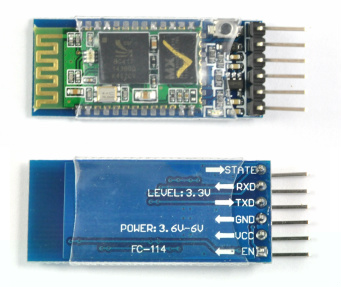
\includegraphics[width=8cm, height=6cm]{HC-05.jpg}
					\caption{}
				\end{figure}